\documentclass[12pt]{article}

\usepackage[utf8]{inputenc}
\usepackage{amsmath}
\usepackage{graphicx}
\usepackage{hyperref}
\usepackage[backend=biber,style=numeric]{biblatex}
\addbibresource{references.bib}

\title{My First LaTeX Document}
\author{Your Name}
\date{\today}

\begin{document}

\maketitle

\section{Introduction}

Hello, world! This is my first document written in \LaTeX.


\section{Math Example}

Here’s an equation:

\[
E = mc^2
\]

\section{Sample figure}

Here is an image:

\begin{figure}[h]

\centering
    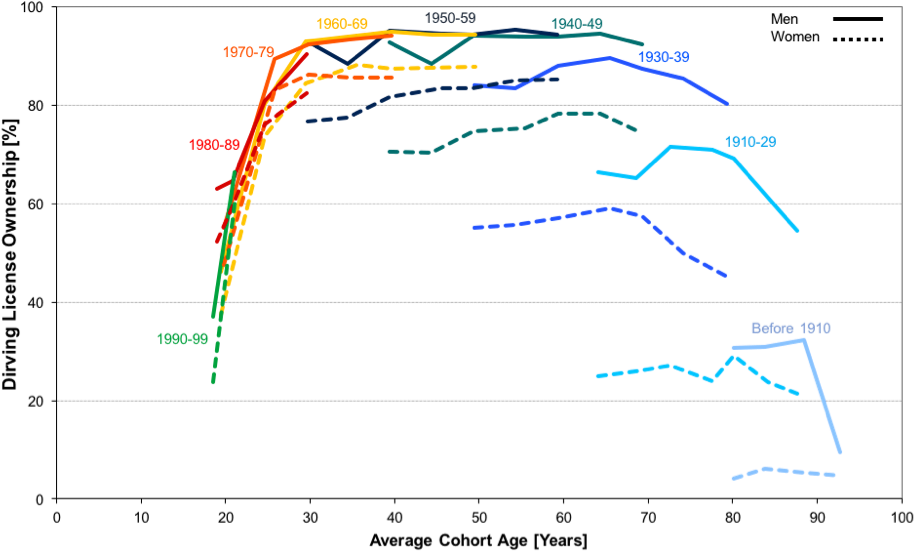
\includegraphics[width=0.7\linewidth]{images/figure1.png}
    \caption{Sample figure}
    \label{fig:sample}
\end{figure}


\section{Conclusion}

\section{Bibliography Demo}

Knuth wrote the definitive book on \TeX{} \cite{knuth1984texbook}.

\printbibliography

Thanks for reading!
\end{document}

